%!TEX program = xelatex

\documentclass[11pt,titlepage]{report}
%!TEX root = main.tex

\usepackage[T1]{fontenc}
\usepackage{lmodern}
\usepackage[svgnames]{xcolor}
\usepackage{fontspec} % XeLaTeX required!
\usepackage{graphicx}
\usepackage{circuitikz}
\usepackage{tikz}
\usepackage{pifont}
\usepackage[some]{background}
\usepackage{xltxtra} 
\usepackage{setspace}
\usepackage[absolute]{textpos}
\usepackage[latin1]{inputenc}
\usepackage[english]{babel}
\usepackage{graphicx}
\usepackage{wrapfig}
\usepackage{fullpage}
\usepackage[margin=1in]{geometry}
\usepackage{float}
\usepackage{url}
\usepackage{multicol}
\usepackage{hyperref}
\usepackage{titlepic}
\usepackage{standalone}
\usepackage{siunitx}
\usepackage{booktabs}
\usepackage{amsmath}
\usepackage{unicode-math}
\usepackage{verbatim}
\usepackage{enumitem}
\usepackage{listings}
\usepackage{multirow}
\usepackage{pgfplots}
\pgfplotsset{compat=1.8}
\usepackage{caption} 
\usepackage[parfill]{parskip}
\usepackage{import}
\usepackage[backend=bibtexu,texencoding=utf8,bibencoding=utf8,style=ieee,sortlocale=en_GB,language=auto]{biblatex}
\usepackage[strict,autostyle]{csquotes}
\usepackage[final]{pdfpages}
\usepackage{subcaption}
\usepackage{ifplatform}
%\captionsetup[table]{skip=10pt}


% Fix for includepdf bug in Mac OS X
\newcommand{\insertpdfpath}[1]{
	\ifwindows
	\newcommand{\insertpdf}[2]{\includepdf[pages=##1]{##2}}
	\else
	\newcommand{\insertpdf}[2]{\includepdf[pages=##1]{#1/##2}}
	\fi
}

%set fonts
\setmainfont[Ligatures=TeX]{Myriad Pro}
\setmathfont{Asana Math}
\setmonofont{Lucida Console}

\usepackage{titlesec, color}
\renewcommand{\familydefault}{\sfdefault} %set font family
\renewcommand{\arraystretch}{1.2} %set table vertical spacing
\setlength\parindent{0pt} %no paragraph indent
\hypersetup{ %setup hyperlinks
    colorlinks,
    citecolor=black,
    filecolor=black,
    linkcolor=black,
    urlcolor=black
}

%redesign chapter headings
\definecolor{gray75}{gray}{0.75}
\newcommand{\chapternumber}{\thechapter}
\newcommand{\hsp}{\hspace{20pt}}
\titleformat{\chapter}[hang]{\Huge\bfseries}{\chapternumber\hsp\textcolor{gray75}{|}\hsp}{0pt}{\Huge\bfseries}

%Redefine appendix headers
\renewcommand{\appendixname}{Appendix}
\renewcommand{\appendixtocname}{Appendices}
\renewcommand{\appendixpagename}{Appendices}

%For code listings
\definecolor{black}{rgb}{0,0,0}
\definecolor{browntags}{rgb}{0.65,0.1,0.1}
\definecolor{bluestrings}{rgb}{0,0,1}
\definecolor{graycomments}{rgb}{0.4,0.4,0.4}
\definecolor{redkeywords}{rgb}{1,0,0}
\definecolor{bluekeywords}{rgb}{0.13,0.13,0.8}
\definecolor{greencomments}{rgb}{0,0.5,0}
\definecolor{redstrings}{rgb}{0.9,0,0}
\definecolor{purpleidentifiers}{rgb}{0.01,0,0.01}


\lstdefinestyle{csharp}{
language=[Sharp]C,
showspaces=false,
showtabs=false,
breaklines=true,
showstringspaces=false,
breakatwhitespace=true,
escapeinside={(*@}{@*)},
columns=fullflexible,
commentstyle=\color{greencomments},
keywordstyle=\color{bluekeywords}\bfseries,
stringstyle=\color{redstrings},
identifierstyle=\color{purpleidentifiers},
basicstyle=\ttfamily\small}

\lstdefinestyle{c}{
language=C,
showspaces=false,
showtabs=false,
breaklines=true,
showstringspaces=false,
breakatwhitespace=true,
escapeinside={(*@}{@*)},
columns=fullflexible,
commentstyle=\color{greencomments},
keywordstyle=\color{bluekeywords}\bfseries,
stringstyle=\color{redstrings},
identifierstyle=\color{purpleidentifiers},
}

\lstdefinestyle{matlab}{
language=Matlab,
showspaces=false,
showtabs=false,
breaklines=true,
showstringspaces=false,
breakatwhitespace=true,
escapeinside={(*@}{@*)},
columns=fullflexible,
commentstyle=\color{greencomments},
keywordstyle=\color{bluekeywords}\bfseries,
stringstyle=\color{redstrings},
identifierstyle=\color{purpleidentifiers}
}

\lstdefinestyle{vhdl}{
language=VHDL,
showspaces=false,
showtabs=false,
breaklines=true,
showstringspaces=false,
breakatwhitespace=true,
escapeinside={(*@}{@*)},
columns=fullflexible,
commentstyle=\color{greencomments},
keywordstyle=\color{bluekeywords}\bfseries,
stringstyle=\color{redstrings},
identifierstyle=\color{purpleidentifiers}
}

\lstdefinestyle{xaml}{
language=XML,
showspaces=false,
showtabs=false,
breaklines=true,
showstringspaces=false,
breakatwhitespace=true,
escapeinside={(*@}{@*)},
columns=fullflexible,
commentstyle=\color{greencomments},
keywordstyle=\color{redkeywords},
stringstyle=\color{bluestrings},
tagstyle=\color{browntags},
morestring=[b]",
  morecomment=[s]{<?}{?>},
  morekeywords={xmlns,version,typex:AsyncRecords,x:Arguments,x:Boolean,x:Byte,x:Char,x:Class,x:ClassAttributes,x:ClassModifier,x:Code,x:ConnectionId,x:Decimal,x:Double,x:FactoryMethod,x:FieldModifier,x:Int16,x:Int32,x:Int64,x:Key,x:Members,x:Name,x:Object,x:Property,x:Shared,x:Single,x:String,x:Subclass,x:SynchronousMode,x:TimeSpan,x:TypeArguments,x:Uid,x:Uri,x:XData,Grid.Column,Grid.ColumnSpan,Click,ClipToBounds,Content,DropDownOpened,FontSize,Foreground,Header,Height,HorizontalAlignment,HorizontalContentAlignment,IsCancel,IsDefault,IsEnabled,IsSelected,Margin,MinHeight,MinWidth,Padding,SnapsToDevicePixels,Target,TextWrapping,Title,VerticalAlignment,VerticalContentAlignment,Width,WindowStartupLocation,Binding,Mode,OneWay,xmlns:x}
}

\lstdefinestyle{matlab}{
language=Matlab,
showspaces=false,
showtabs=false,
breaklines=true,
showstringspaces=false,
breakatwhitespace=true,
escapeinside={(*@}{@*)},
columns=fullflexible,
commentstyle=\color{greencomments},
keywordstyle=\color{bluekeywords}\bfseries,
stringstyle=\color{purpleidentifiers},
identifierstyle=\color{purpleidentifiers}
}

%defaults
\lstset{
basicstyle=\ttfamily\small,
extendedchars=false,
numbers=left,
numberstyle=\ttfamily\tiny,
stepnumber=1,
tabsize=4,
numbersep=5pt
}
\addbibresource{../../library/bibliography.bib}

\begin{document}

\chapter{System integration}
\label{ch:integration}
Now that we have discussed all of the individual subsystem designs, we can describe how these were put together for the final design. The system was developed to achieve optimal performance during the mid-term challenge, which consists of charging the supercapacitor bank to \SI{20}{V} with our contactless charging system (not mounted on KITT), as well as letting KITT drive to a position as close to a wall as possible, in the least possible amount of time. \\
For the charging system, \textit{integration} was not really necessary, since the subsystem itself has proved itself working just fine already as described in Chapter~\ref{ch:charging}. During the mid-term challenge, we were able to charge the capacitor bank to little under \SI{20}{V} in around \SI{3.5}{minutes}, before the overcurrent protection kicked in and the overvoltage buffer started buzzing softly.
\\
The control system, however, still needed some work. We described the physical and mathematical background of our design in the previous chapter (Chapter~\ref{ch:control}), but every design needs an implementation.

\section{The user interface}
For controlling KITT in a simple way and at the same time being able to view live sensor and calculated state data, we have implemented the controller in conjunction with a graphical user interface (GUI). This GUI provides access to key features in controlling KITT, like the target distance and some model parameters, as well as a dashboard which displays KITT's current state, such as the current position, battery voltage and the likes. This way we are able to debug and adapt the underlying control routines more easily, which, in theory, increases development efficiency.
\\\\
The control routines themselves are essentially the previously derived state equations wrapped in the programming language of our choice, as well as some functions that help obtaining the required data for evaluating these equations. The user interface only provides an easy way to influence these procedures (like modifying model parameters), and displays some of the obtained data in an easy-to-read way. A rough diagram of the program's structure is shown in Figure~\ref{fig:int-controller}. For flexibility, we developed two main control programs, one in MATLAB, which provides rapid prototyping in a cross-platform environment and one in Microsoft's .NET (C\#), which was supposed to bring us better performance and a better looking GUI.

\usetikzlibrary{shapes,arrows}
\tikzstyle{block} = [
	rectangle,
	draw,
	fill=blue!20, 
    text width=7em, 
    text centered,
    rounded corners,
    minimum height=4em
]
\tikzstyle{every edge} = [
	draw,
	>=triangle 90
]

\begin{figure}[H]
	\centering
	\begin{tikzpicture}[node distance = 5cm, auto]
		% Nodes
		\node [block] (gui) {User interface};
		\node [block, below left= 3cm of gui] (comm) {Communications};
		\node [block, above left= 3cm of gui] (control) {Control};
		\coordinate[right= 3cm of gui] (1);
		\coordinate[left= 3cm of comm] (2);
		% Edges
		\path (1) edge [->] node {User interaction} (gui.east);
		\path ([xshift=-7]gui.north) edge [->] node [left, near start]{Influence control} ([yshift=-7]control.east);
		\path ([yshift=7]control.east) edge [->] node [right, near start]{Display state data} ([xshift=7]gui.north);
		\path ([xshift=-7]gui.south) edge [->] node [left, near start]{Connect with KITT} ([yshift=7]comm.east);
		\path ([yshift=-7]comm.east) edge [->] node [right, near start]{Display KITT's status} ([xshift=7]gui.south);
		\path ([xshift=-7]control.south) edge [->] node [right, very near start]{Control KITT} ([xshift=-7]comm.north);
		\path ([xshift=7]comm.north) edge [->] node [left, very near start]{Obtain sensor data} ([xshift=7]control.south);
		\path ([yshift=7]comm.west) edge [->] node [above]{To KITT} ([yshift=7]2);
		\path ([yshift=-7]2) edge [->] node [below]{From KITT} ([yshift=-7]comm.west);
	\end{tikzpicture}
	\caption{Rough diagram of the structure of the control program}
	\label{fig:int-controller}
\end{figure}

\subsection{MATLAB}
MATLAB provides rapid prototyping, because of the great amount of mathematical operations and concepts (like matrices) available in its scripting language. All concepts were first implemented in MATLAB for testing, after which they could be ported to .NET. One of the drawbacks of MATLAB is that object-oriented programming, e.g. when designing a user interface, can be somewhat cumbersome at times.

\begin{figure}[H]
	\centering
	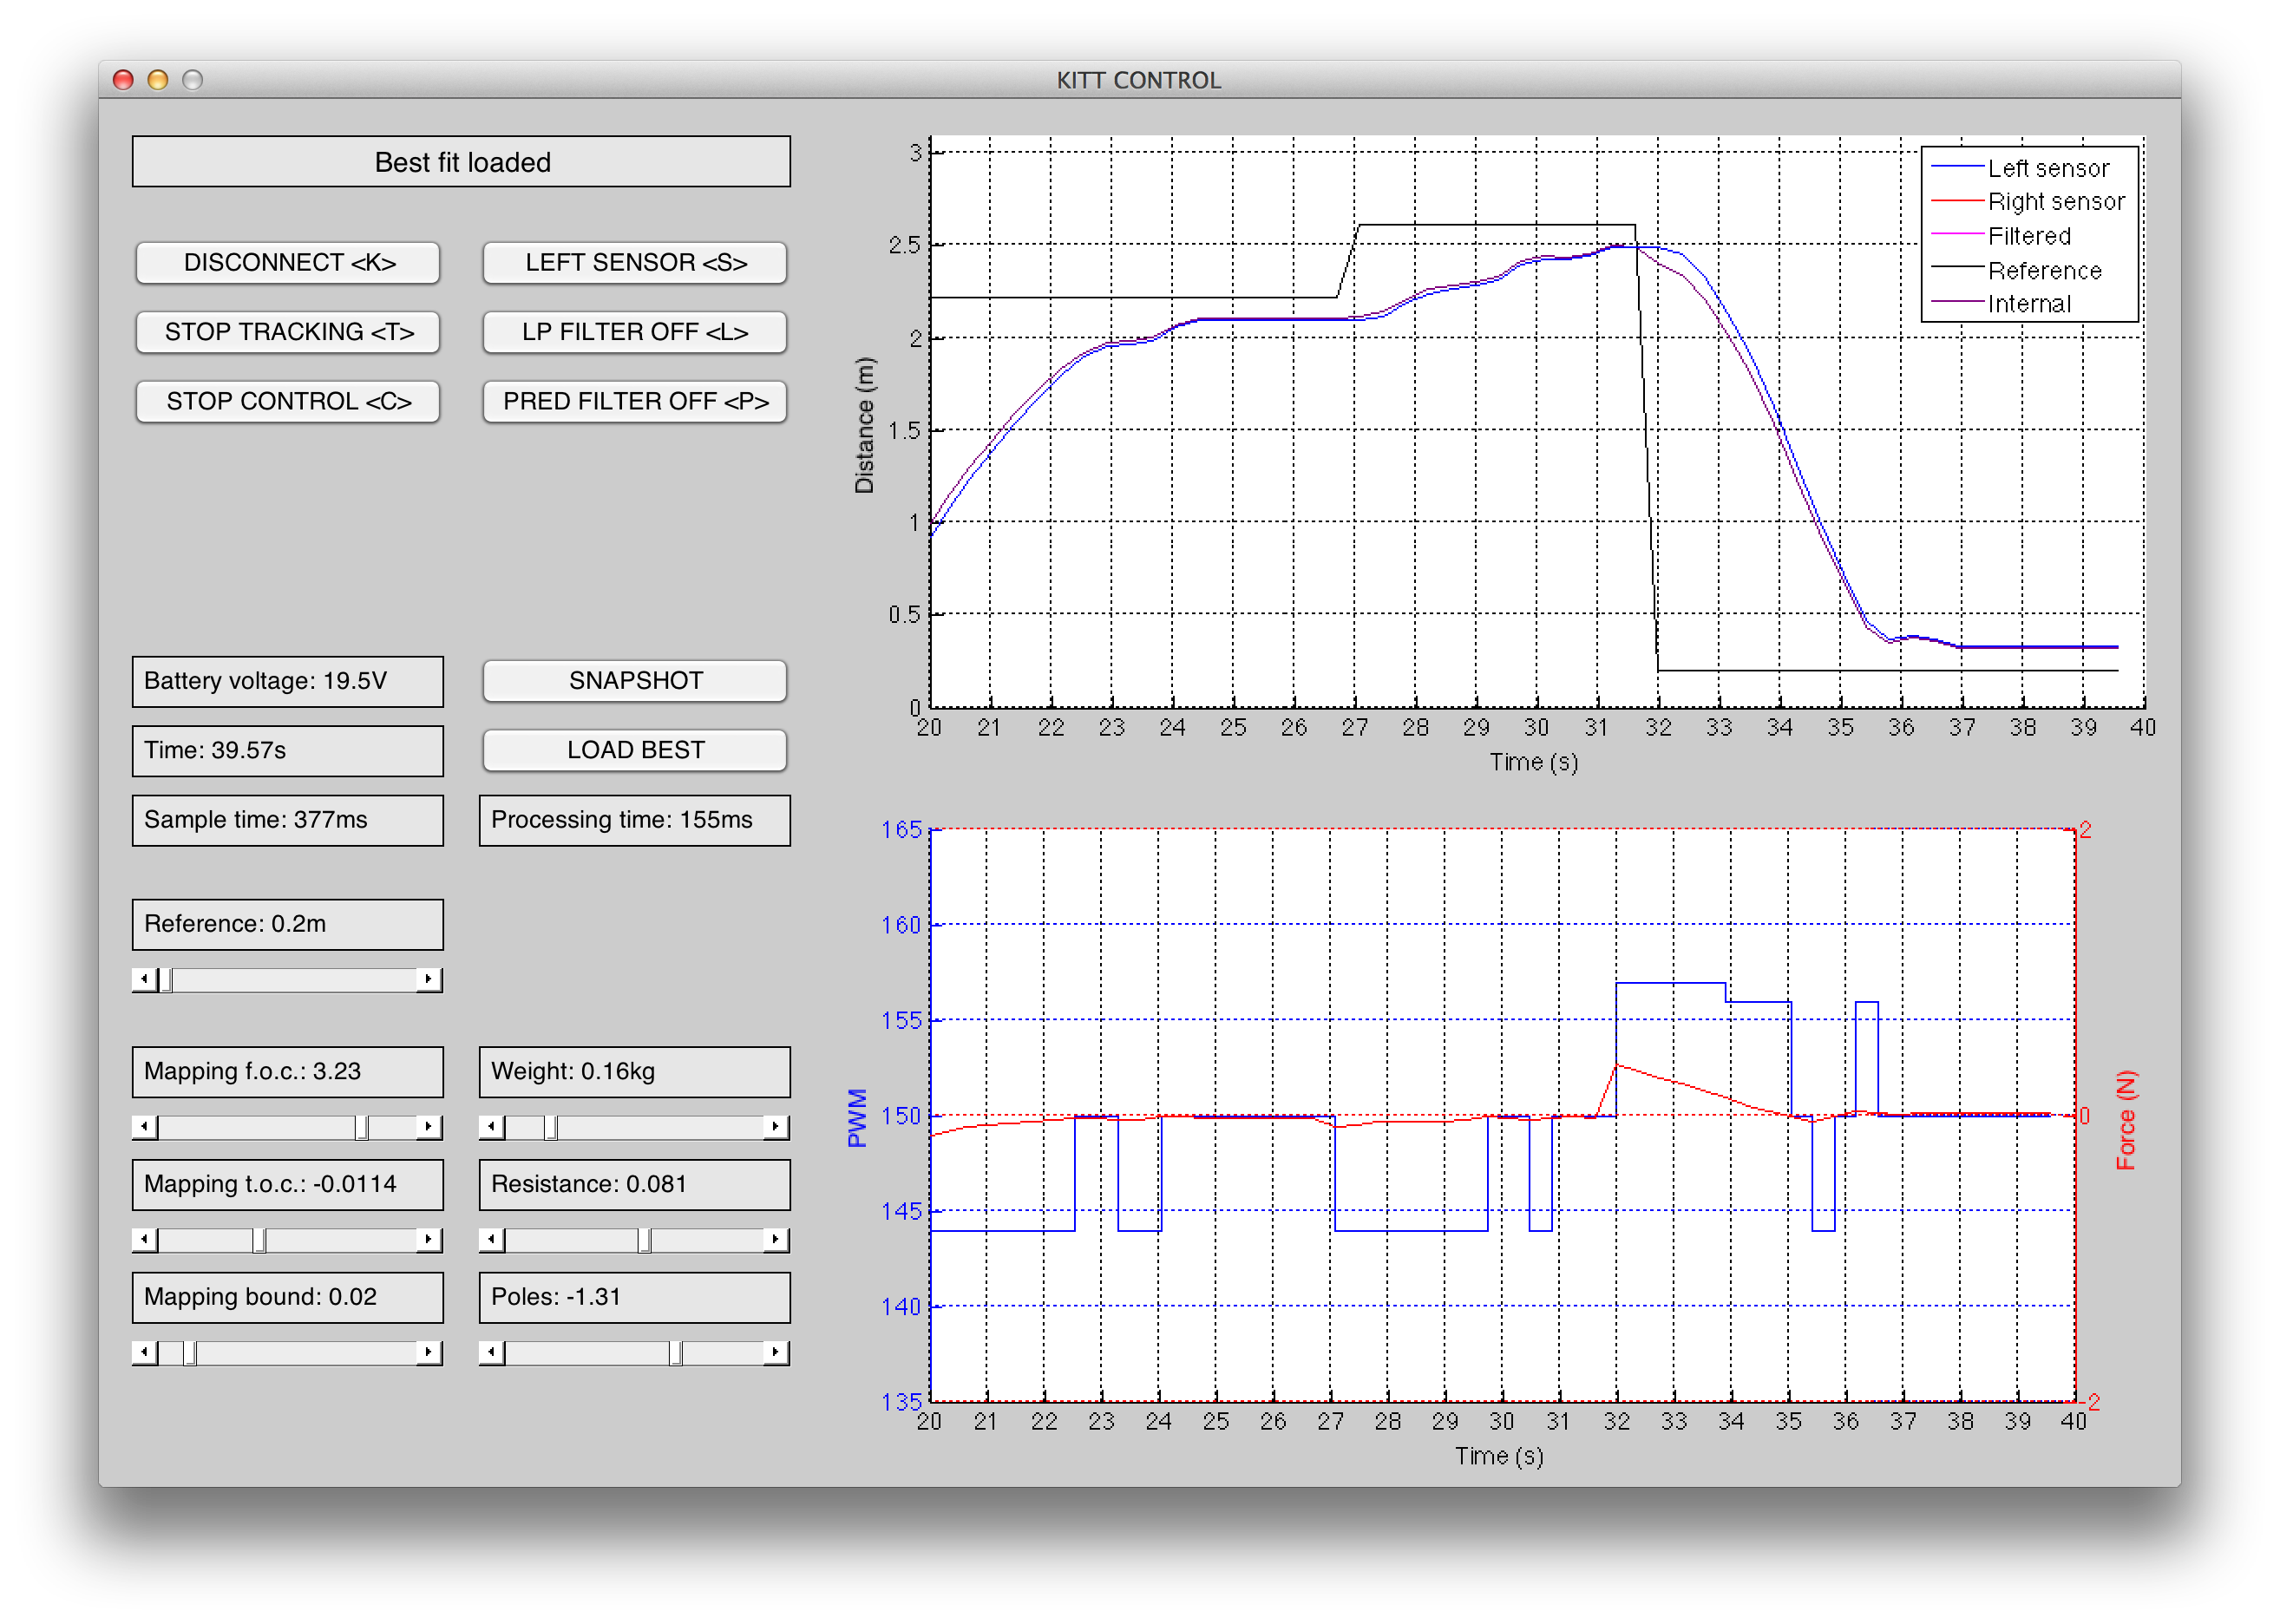
\includegraphics[width=\linewidth]{resource/gui-matlab.png}
	\caption{The MATLAB GUI, KITT is simulated}
	\label{fig:int-gui-matlab}
\end{figure}

Our MATLAB program as shown in Figure~\ref{fig:int-gui-matlab} provides very much configurability, like the ability to change model parameters \textit{on the fly} for directly influencing KITT's behaviour while testing. When KITT behaves in a way that we think is acceptable, we can save the current set of parameters to a file, so that loading them during the next run is possible. It also features two graphs updated in real-time for displaying KITT's output and state data as well as the actual calculated excitation speed. We see that the simulated KITT converges to the reference distance, indicating the controller theoretically works. Tests with the real KITT and the mid-term challenge itself, proved that the controller works in real-life as well.
A small discrepancy we can spot in the behaviour is that the (simulated) KITT does not reach the reference distance but stops at a small distance from it. This is due to the fact that we map every excitation $145 < \text{PWM}(u) < 155$ to zero, which essentially decreases the resolution of the control process. This behaviour will return in the C\# GUI, since the same mapping function is used in it. To overcome this, we could decide to map $145 < \text{PWM}(u) < 155$, or a range somewhat smaller, to \num{144} or \num{156} in stead of zero, so KITT will always drive when not on, or at least really close to his target position. This could, however, result in bouncy behaviour, caused by ever continuing overshoot due to the excitation being too high to realize the required accuracy. 

\begin{figure}[H]
	\centering
	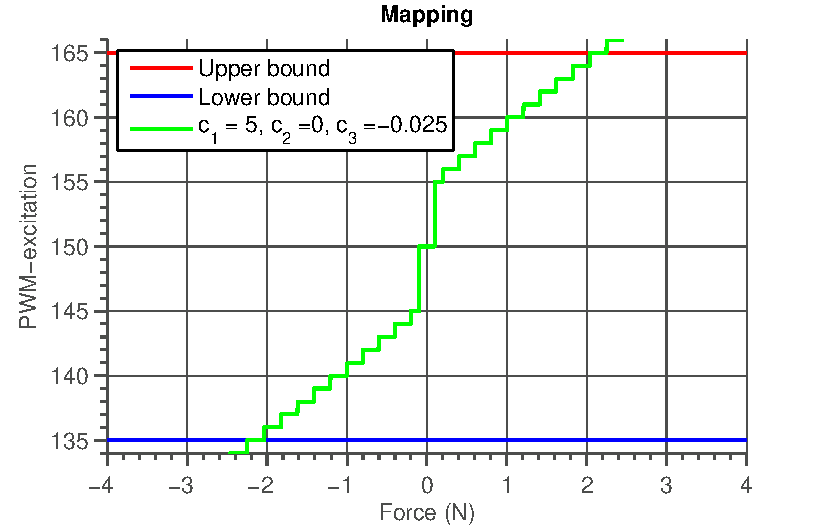
\includegraphics[width=0.7\linewidth]{resource/mapping.pdf}
	\caption{An example of force to PWM excitation mapping using a third order polynomial with arbitrary coefficients}
	\label{fig:int-mapping}
\end{figure}

For testing the controller of course a serial connection for sending and retrieving data from KITT was required. To this end a simple script utilizing MATLAB's built-in serial functionality was created. Using this script we noticed very high communication latencies from \SI{200}{ms} to as high as \SI{600}{ms}. Because this latency makes accurate control of KITT very hard, a second serial module was written in native C-code. This seemed to decrease the latency somewhat, but the line between parking KITT around \SI{20}{cm} from the wall and driving straight into the wall was still very thin.
\\
The source code of the MATLAB GUI can be found in Appendix~\ref{appsec:kitt-mat}. Source of the serial module is found in Appendix~\ref{appsec:kitt-serial-c}.

\subsection{.NET}
Our .NET implementation has the same mathematical backbone as the MATLAB GUI. It is structured very differently. Each subsystem, like control, user input, serial communication and status data storage is contained in a separate \textit{class}. Apart from this it provides the possibility to control KITT manually via mouse and keyboard input. It also handles serial communication asynchronously. Whenever the program receives data from KITT, it will directly process it and store the new state values in a set of variables (in a class) that can be accessed by all other classes at each given time. This way the program does not have to wait on KITT during execution, which should theoretically speed up the process.

\begin{figure}[H]
	\centering
	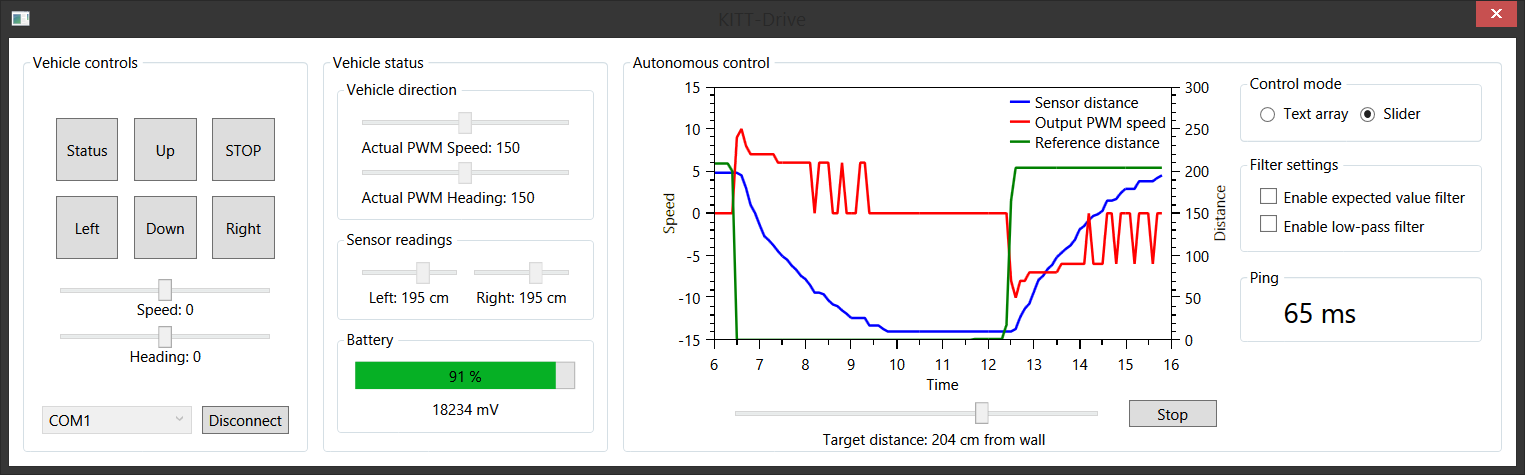
\includegraphics[width=\linewidth]{resource/gui-dotnet.png}
	\caption{The .NET GUI, KITT is simulated}
	\label{fig:int-gui-dotnet}
\end{figure}

In Figure~\ref{fig:int-gui-dotnet} the .NET GUI is shown in action, we see that the simulated KITT converges to the the given reference distance as expected, including a little offset as explained earlier. In tests with this program with a real KITT, we observed latencies of around \SI{20}{ms}, which is significantly lower than the latencies using MATLAB. This renders the overall performance of the .NET program higher.
\\
The source code of the .NET GUI can be found in Appendix~\ref{appsec:kitt-drive-dotnet}.

\section{Testing the programs}
Most ideally we would perform our tests on an actual KITT car, but since this was not always possible, we wrote programs to simulate KITT's behaviour with in both MATLAB and C\#. These programs utilize a \textit{virtual} or \textit{pseudo} COM-port. This way the simulator can operate on, for example COM1, sending data to the control program via COM0 and vice versa. This provides an easy way to observe an estimate of the performance of the control system with a real KITT.
\\
Source code of both programs can be found in Appendix~\ref{appsubsubsec:kitt-mat-kitt-c-emu} (MATLAB) and \ref{appsec:serialapp} (C\#).

\end{document}